\phantomsection
\section*{Anhang}
\addcontentsline{toc}{section}{Anhang}

\subsection*{Technische Umsetzung des UAP-Generierungsprozesses}

Die technische Umsetzung des Prozesses zur Generierung der \acrshort{uap} Bilder ist in der folgenden Grafik dargestellt:

\begin{figure}[H]
    \centering
    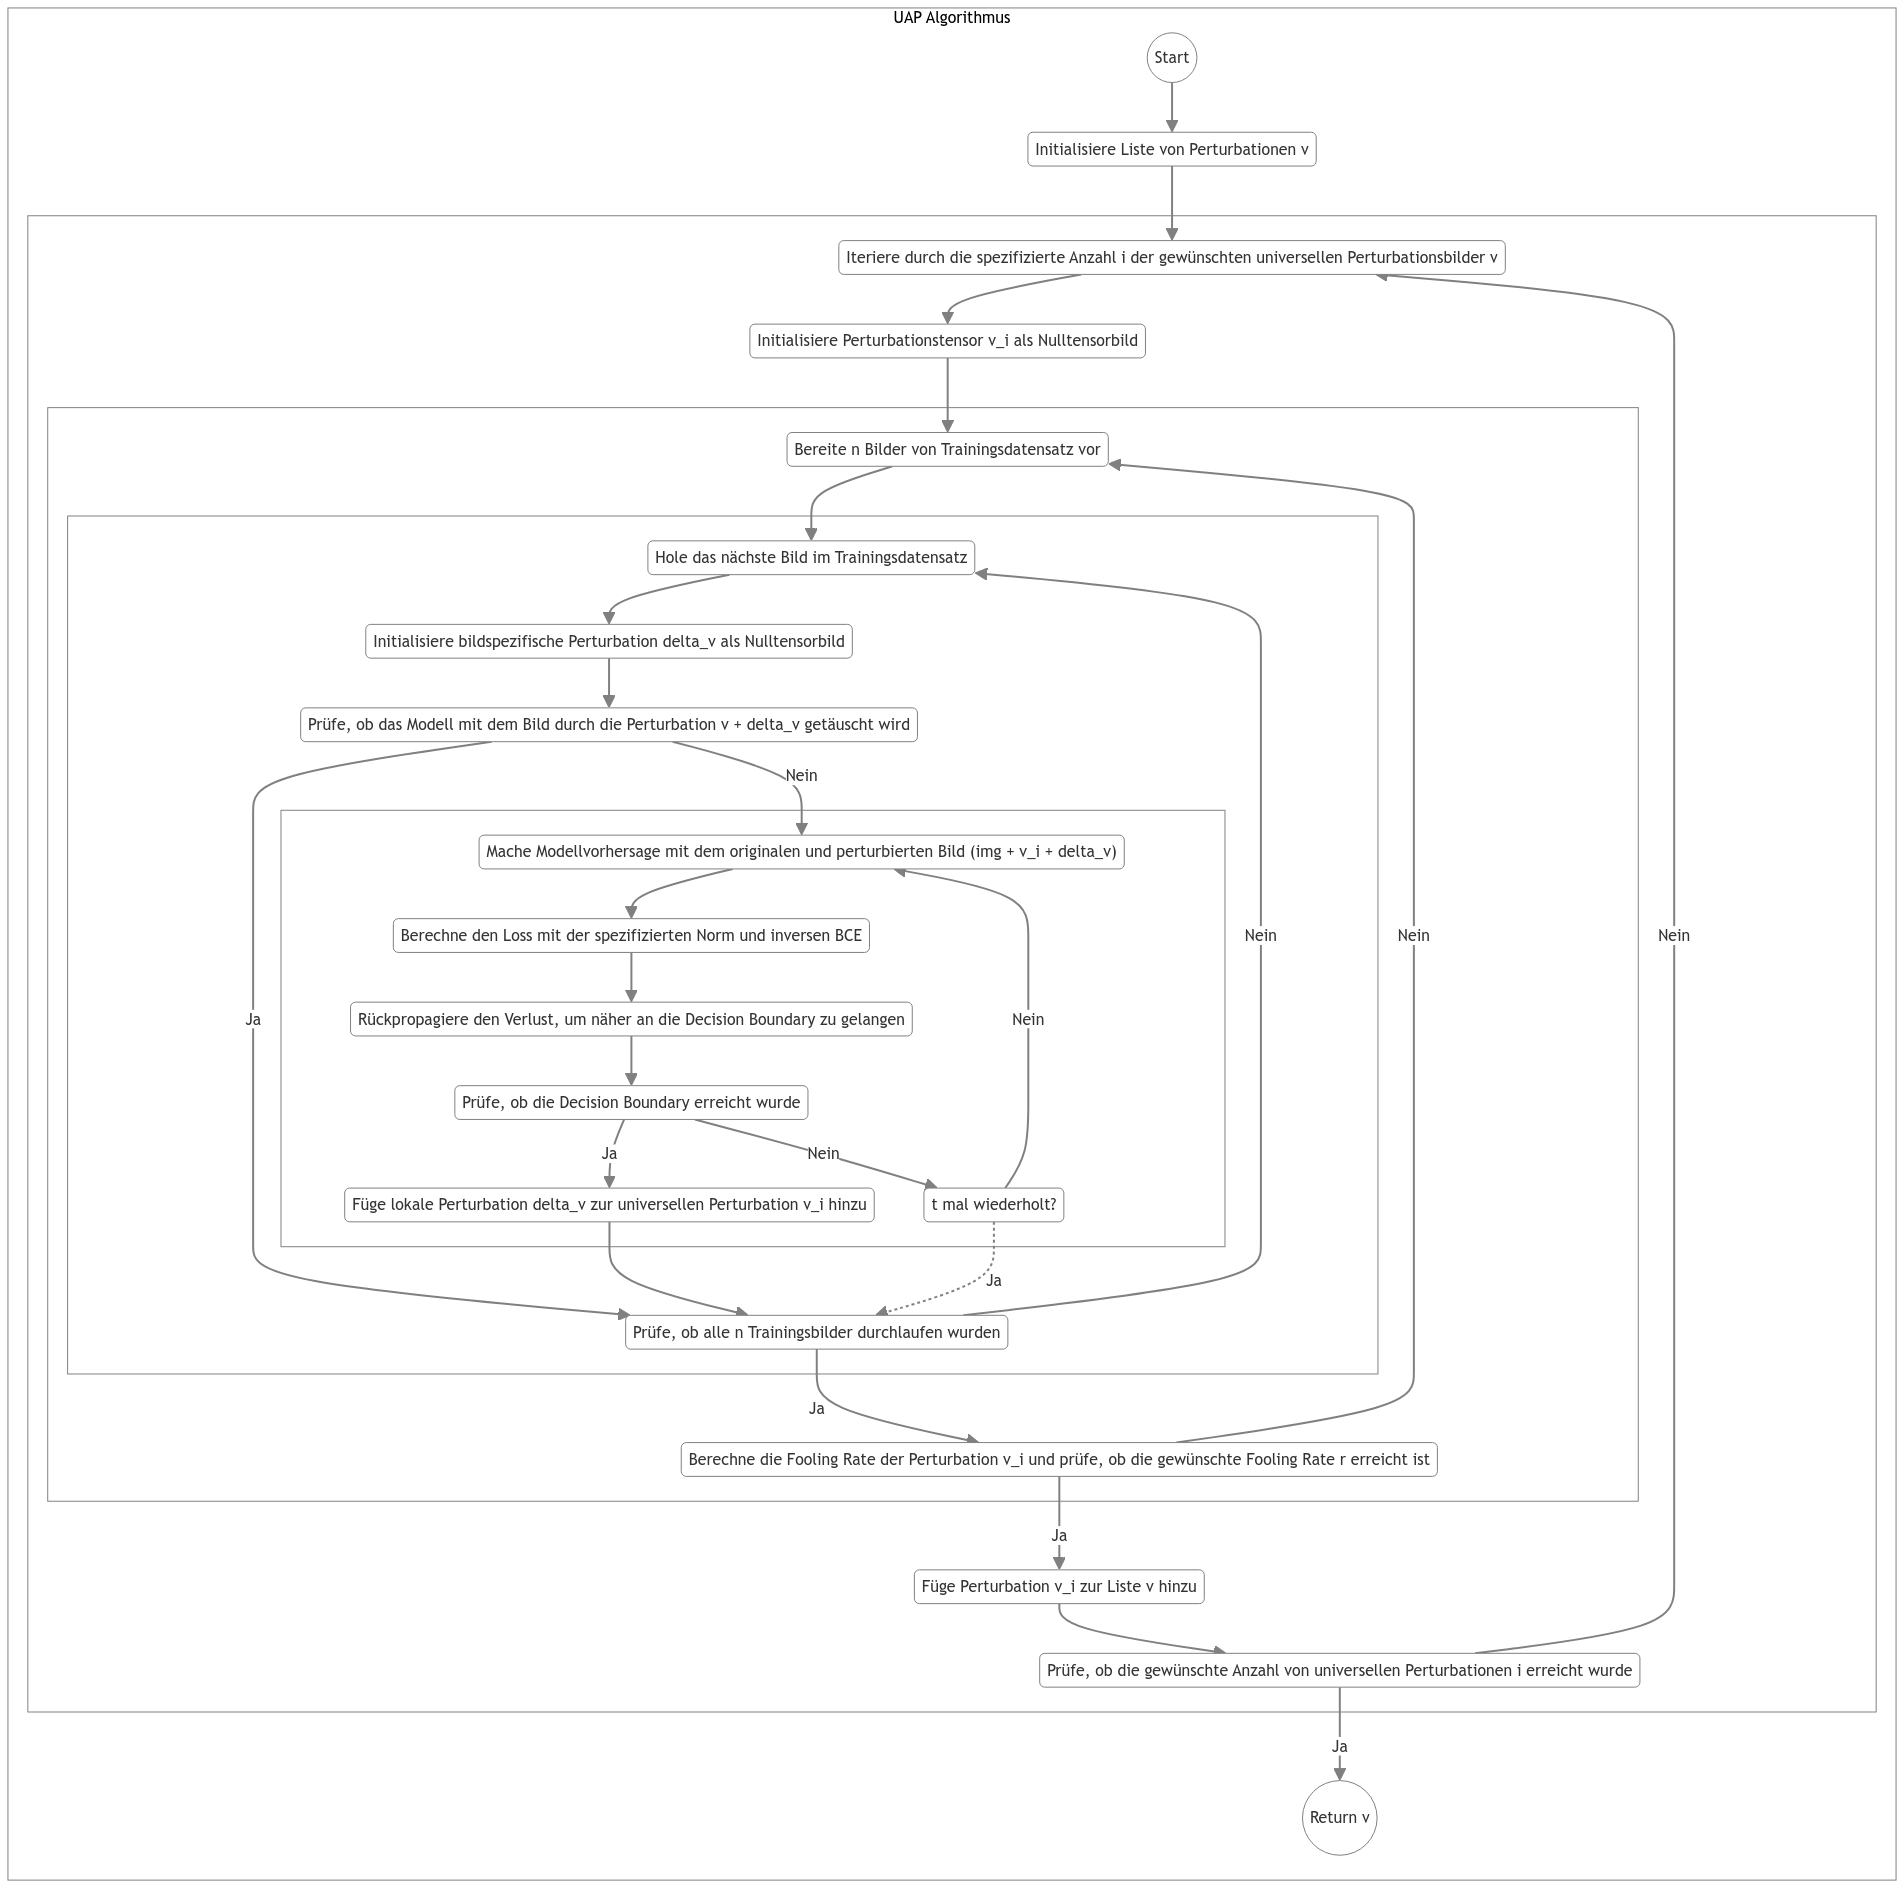
\includegraphics[width=\linewidth]{01-images/04-methodik/UAP_ALG.png}
    \caption{Schematische Darstellung des UAP-Generierungsprozesses}
    \label{fig:05-uap_algorithm}
\end{figure}

\newpage

\subsection*{Technische Umsetzung der Adversarial Training Pipeline}

\begin{algorithm}
\caption{Pipeline zur Generierung von universelle adversarial Perturbationen}
\label{alg:UAP_Adversarial_Training_Pipeline}
\begin{algorithmic}[1]
\STATE Modell $f(\cdot)$ laden
\FOR{Anzahl Robustifizierungen $n_{\text{robustifications}}$}
    \STATE Generierung der \acrshort{uap}s (Algorithmus \ref{algo:UAP Algorithmus})
    \STATE Inferenz auf den Validierungsdaten $X_{\text{val}}$ und Testdaten $X_{\text{test}}$ ($p_{\text{adv}}$=0.0)
    \FOR{jede \acrshort{uap}}
        \STATE Inferenz auf den Validierungsdaten $X_{\text{val}}$ und Testdaten $X_{\text{test}}$ mit \acrshort{uap} ($p_{\text{adv}}$=1.0)
    \ENDFOR
    \STATE Modell finetuning mittels \acrshort{uap}s ($X_{\text{train}}$, $X_{\text{val}}$, random selection, $p_{\text{adv},\text{train}}$=0.5, \\
    $p_{\text{adv},\text{val}}$=0.5)
    \STATE Laden des besten Modellcheckpoints
    \STATE Inferenz auf den Validierungsdaten $X_{\text{val}}$ und Testdaten $X_{\text{test}}$ mit dem robustifiziertem Modell ($p_{\text{adv}}$=0.0)
    \FOR{jede \acrshort{uap}}
        \STATE Inferenz auf den Validierungsdaten $X_{\text{val}}$ und Testdaten $X_{\text{test}}$ mit \acrshort{uap} mit dem robustifizierem Modell ($p_{\text{adv}}$=1.0)
    \ENDFOR
\ENDFOR
\end{algorithmic}
\end{algorithm}

Eine vereinfachte, visualisierte Version der Adversarial Training Pipeline ohne Validierungsdatensatz:

\begin{figure}[H]
    \centering
    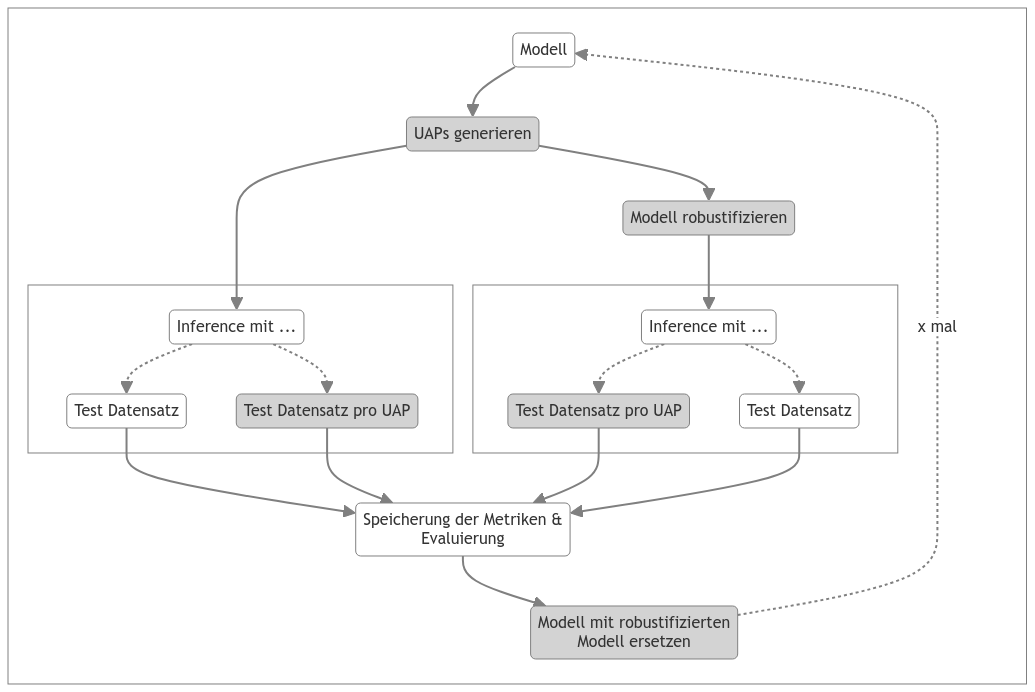
\includegraphics[width=\linewidth]{01-images/04-methodik/robustifizierungs-pipeline.png}
    \caption{Übersicht der Evaluierungspipeline}
    \label{fig:Evaluierungspipeline}
\end{figure}

\newpage

\subsection*{Weitere Analysen}
\subsubsection*{Feature Maps \& PCA} \label{chap:FeatureMaps-TestProblemEda3-mri}
Im Rahmen unserer Analyse nutzen wir ein ResNet50-Modell, das zum einen durch PyTorch vorab trainiert und zum anderen speziell auf unseren Datensatz angepasst. Besonderes Augenmerk liegt auf der Featureextraktion aus dem vorletzten Layer des Modells, direkt vor dem Klassifikationslayer. Die in diesem Schritt gewonnenen Vektoren, auch als Feature Maps bekannt, durchlaufen einer PCA Dimensionsreduktion. Ziel dieser Reduktion ist es, die Dimensionalität der Daten auf zwei Dimensionen zu reduzieren, um eine Visualisierung der verschiedenen Datenpartitionen zu ermöglichen. Die Interpretation erweist sich als sehr komplex und die Ergebnisse sind nur schwer zu interpretieren. 

\paragraph*{Covid}

\begin{figure}[H]
    \centering
    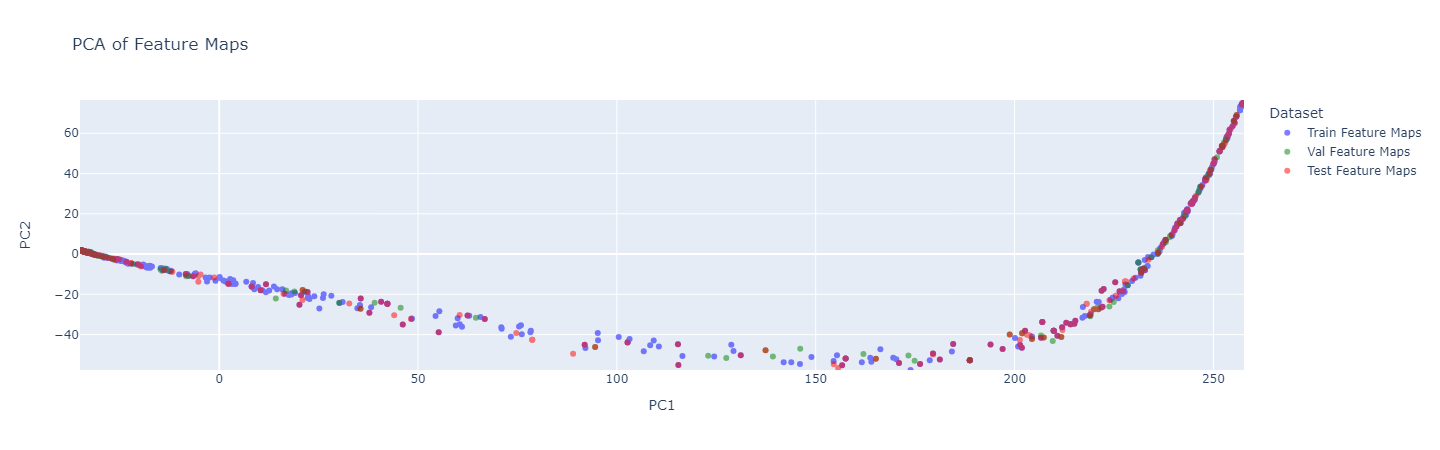
\includegraphics[width=\linewidth]{01-images/06-ending/covidx-all-feautremap-pca-ourmodel-resnet50.png}
    \caption{Hauptkomponenten der PCA-Analyse von zweitletzten Covid Featuremaps Layer eines vortrainierten ResNet50-Modells für Covid}
    \label{fig:covidx-feautremap-pca-ourmodel-resnet50}
\end{figure}

\begin{figure}[H]
    \centering
    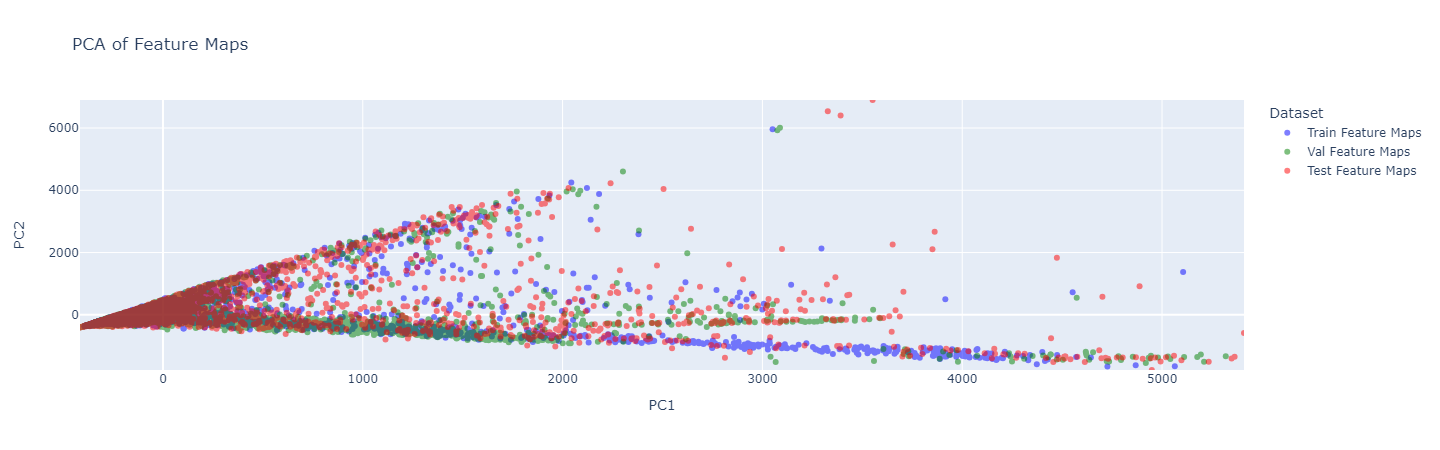
\includegraphics[width=\linewidth]{01-images/06-ending/covidx-all-feautremap-pca-model-resnet50.png}
    \caption{Hauptkomponenten der PCA-Analyse von zweitletzten Covid Featuremaps Layer eines vortrainierten ResNet50-Modells}
    \label{fig:covidx-feautremap-pca-model-resnet50}
\end{figure}


\paragraph*{Hirntumor}

\begin{figure}[H]
    \centering
    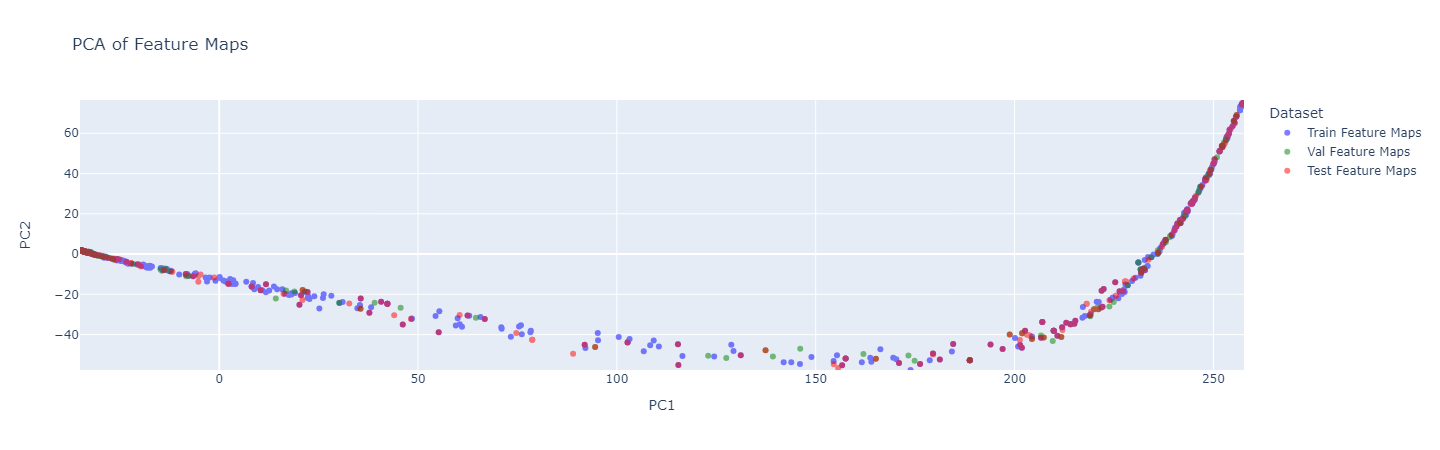
\includegraphics[width=\linewidth]{01-images/06-ending/brain-all-feautremap-pca-ourmodel-resnet50.png}
    \caption{Hauptkomponenten der PCA-Analyse von zweitletzten Hirntumor Featuremaps Layer eines vortrainierten ResNet50-Modells für Hirntumor}
    \label{fig:brain-feautremap-pca-ourmodel-resnet50}
\end{figure}

\begin{figure}[H]
    \centering
    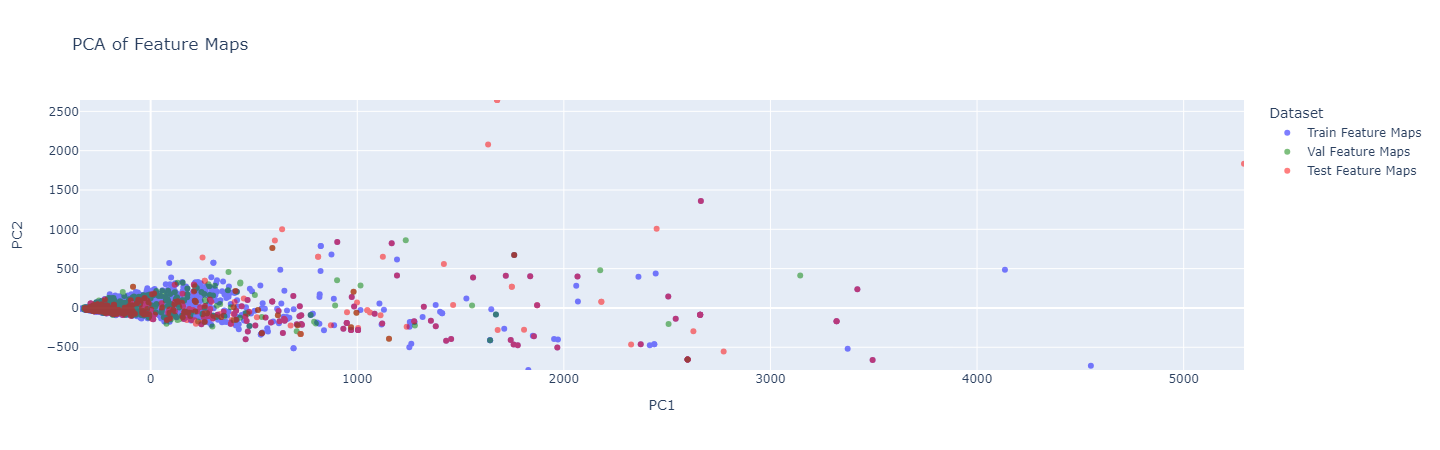
\includegraphics[width=\linewidth]{01-images/06-ending/brain-all-feautremap-pca-model-resnet50.png}
    \caption{Hauptkomponenten der PCA-Analyse von zweitletzten Hirntumor Featuremaps Layer eines vortrainierten ResNet50-Modells}
    \label{fig:brain-feautremap-pca-model-resnet50}
\end{figure}

\newpage

% Übrige UAP
\subsection*{Übrige Universelle Adversarial Perturbation} \label{appendix:übrige-uaps}
Hier werden die übrig gebliebenen UAP Indexe für jede Robustifikationslevel, Modell und Datensatz visualisiert. 

% ResNet18 Covid
\subsubsection*{UAP von ResNet18 - Covidx CXR-4} 
\begin{figure}[H]
    \centering
    \foreach \y in {0,1,2,3,4} {%
        \text{Entwicklung der UAP (Index \y) durch Adversarial Attack und Adversarial Training}\\
        \foreach \x in {0,...,9} {%
            \begin{subfigure}{0.095\linewidth}
                \centering
                \includegraphics[height=1\linewidth]{01-images/05-resultate/uap_resnet18/uap\y-resnet18-covidx_data-n200-robustificationslevel\x.png}
            \end{subfigure}\hfill%
        }
    }
    \caption{Übrige Generierte UAPs der mit ResNet18 trainierten Covidx CXR-4 Datensätze nach jedem Robustifikationslevel durch Adversarial Training von links nach rechts für alle Indizes.}
    \label{fig-appendix:uap-resnet18-covid-rest}
\end{figure}

% ResNet18 MRI
\subsubsection*{UAP von ResNet18 - Hirntumor}
\begin{figure}[H]
    \centering
    \foreach \y in {0,1,2,3,4} {%
        \text{Entwicklung der UAP (Index \y) durch Adversarial Attack und Adversarial Training}\\
        \foreach \x in {0,...,6} {%
            \begin{subfigure}{0.095\linewidth}
                \centering
                \includegraphics[height=1\linewidth]{01-images/05-resultate/uap_resnet18/uap\y-resnet18-mri_data-n200-robustificationslevel\x.png}
            \end{subfigure}\hfill%
        }
    }
    \caption{Übrige Generierte UAPs der mit ResNet18 trainierten Hirntumor Datensatz nach jedem Robustifikationslevel durch Adversarial Training von links nach rechts für alle Indizes.}
    \label{fig-appendix:uap-resnet18-hirntumor-rest}
\end{figure}

% ResNet50 Covid
\subsection*{UAP von ResNet50 - Covidx CXR-4}
\begin{figure}[H]
    \centering
    \foreach \y in {0,1,2,3,4} {%
        \text{Entwicklung der UAP (Index \y) durch Adversarial Attack und Adversarial Training}\\
        \foreach \x in {0,...,9} {%
            \begin{subfigure}{0.095\linewidth}
                \centering
                \includegraphics[height=1\linewidth]{01-images/05-resultate/uap_resnet50/uap\y-resnet50-covidx_data-n200-robustificationslevel\x.png}
            \end{subfigure}\hfill%
        }
    }
    \caption{Übrige Generierte UAPs der mit ResNet50 trainierten Covidx CXR-4 Datensätze nach jedem Robustifikationslevel durch Adversarial Training von links nach rechts für alle Indizes.}
    \label{fig-appendix:uap-resnet50-covid-rest}
\end{figure}

% ResNet50 MRI
\subsubsection*{UAP von ResNet50 - Hirntumor}
\begin{figure}[H]
    \centering
    \foreach \y in {0,1,2,3,4} {%
        \text{Entwicklung der UAP (Index \y) durch Adversarial Attack und Adversarial Training}\\
        \foreach \x in {0,...,9} {%
            \begin{subfigure}{0.095\linewidth}
                \centering
                \includegraphics[height=1\linewidth]{01-images/05-resultate/uap_resnet50/uap\y-resnet50-mri_data-n200-robustificationslevel\x.png}
            \end{subfigure}\hfill%
        }
    }
    \caption{Übrige Generierte UAPs der mit ResNet50 trainierten Hirntumor Datensatz nach jedem Robustifikationslevel durch Adversarial Training von links nach rechts für alle Indizes.}
    \label{fig-appendix:uap-resnet50-hirntumor-rest}
\end{figure}

% EfficientNetV2-M Covid
\subsubsection*{UAP von EfficientNetV2-M - Covidx CXR-4}
\begin{figure}[H]
    \centering
    \foreach \y in {0,1,2,3,4} {%
        \text{Entwicklung der UAP (Index \y) durch Adversarial Attack und Adversarial Training}\\
        \foreach \x in {0,...,9} {%
            \begin{subfigure}{0.095\linewidth}
                \centering
                \includegraphics[height=1\linewidth]{01-images/05-resultate/uap_efficientnet_m/uap\y-efficientnet_v2_m-covidx_data-n200-robustificationslevel\x.png}
            \end{subfigure}\hfill%
        }
    }
    \caption{Übrige Generierte UAPs der mit EfficientNet-V2-M trainierten Covidx CXR-4 Datensätze nach jedem Robustifikationslevel durch Adversarial Training von links nach rechts für alle Indizes.}
    \label{fig-appendix:uap-efficientnetv2m-covid-rest}
\end{figure}

% EfficientNetV2-M MRI
\subsubsection*{UAP von EfficientNetV2-M - Hirntumor}
\begin{figure}[H]
    \centering
    \foreach \y in {0,1,2,3,4} {%
        \text{Entwicklung der UAP (Index \y) durch Adversarial Attack und Adversarial Training}\\
        \foreach \x in {0,...,4} {%
            \begin{subfigure}{0.095\linewidth}
                \centering
                \includegraphics[height=1\linewidth]{01-images/05-resultate/uap_efficientnet_m/uap\y-efficientnet_v2_m-mri_data-n200-robustificationslevel\x.png}
            \end{subfigure}\hfill%
        }
    }
    \caption{Übrige Generierte UAPs der mit EfficientNet-V2-M trainierten Hirntumor Datensatz nach jedem Robustifikationslevel durch Adversarial Training von links nach rechts für alle Indizes.}
    \label{fig-appendix:uap-efficientnetv2m-hirntumor-rest}
\end{figure}

% EfficientNetV2-S Covid
\subsubsection*{UAP von EfficientNetV2-S - Covidx CXR-4}
\begin{figure}[H]
    \centering
    \foreach \y in {0,1,2,3,4} {%
        \text{Entwicklung der UAP (Index \y) durch Adversarial Attack und Adversarial Training}\\
        \foreach \x in {0,...,9} {%
            \begin{subfigure}{0.095\linewidth}
                \centering
                \includegraphics[height=1\linewidth]{01-images/05-resultate/uap_efficientnet_s/uap\y-efficientnet_v2_s-covidx_data-n200-robustificationslevel\x.png}
            \end{subfigure}\hfill%
        }
    }
    \caption{Übrige Generierte UAPs der mit EfficientNet-V2-S trainierten Covidx CXR-4 Datensätze nach jedem Robustifikationslevel durch Adversarial Training von links nach rechts für alle Indizes.}
    \label{fig-appendix:uap-efficientnetv2s-covid-rest}
\end{figure}

% EfficientNetV2-S MRI
\subsubsection*{UAP von EfficientNetV2-S - Hirntumor}
\begin{figure}[H]
    \centering
    \foreach \y in {0,1,2,3,4} {%
        \text{Entwicklung der UAP (Index \y) durch Adversarial Attack und Adversarial Training}\\
        \foreach \x in {0,...,0} {%
            \begin{subfigure}{0.095\linewidth}
                \centering
                \includegraphics[height=1\linewidth]{01-images/05-resultate/uap_efficientnet_s/uap\y-efficientnet_v2_s-mri_data-n200-robustificationslevel\x.png}
            \end{subfigure}\hfill%
        }
    }
    \caption{Übrige Generierte UAPs der mit EfficientNet-V2-S trainierten Hirntumor Datensatz nach jedem Robustifikationslevel durch Adversarial Training von links nach rechts für alle Indizes.}
    \label{fig-appendix:uap-efficientnetv2s-hirntumor-rest}
\end{figure}

% DenseNet169 Covid
\subsubsection*{UAP von DenseNet169 - Covidx CXR-4}
\begin{figure}[H]
    \centering
    \foreach \y in {0,1,2,3,4} {%
        \text{Entwicklung der UAP (Index \y) durch Adversarial Attack und Adversarial Training}\\
        \foreach \x in {0,...,2} {%
            \begin{subfigure}{0.095\linewidth}
                \centering
                \includegraphics[height=1\linewidth]{01-images/05-resultate/uap_densenet169/uap\y-densenet169-covidx_data-n200-robustificationslevel\x.png}
            \end{subfigure}\hfill%
        }
    }
    \caption{Übrige Generierte UAPs der mit DenseNet169 trainierten Covidx CXR-4 Datensätze nach jedem Robustifikationslevel durch Adversarial Training von links nach rechts für alle Indizes.}
    \label{fig-appendix:uap-densenet169-covid-rest}
\end{figure}

% DenseNet169 MRI
\subsubsection*{UAP von DenseNet169 - Hirntumor}
\begin{figure}[H]
    \centering
    \foreach \y in {0,1,2,3,4} {%
        \text{Entwicklung der UAP (Index \y) durch Adversarial Attack und Adversarial Training}\\
        \foreach \x in {0,...,9} {%
            \begin{subfigure}{0.095\linewidth}
                \centering
                \includegraphics[height=1\linewidth]{01-images/05-resultate/uap_densenet169/uap\y-densenet169-mri_data-n200-robustificationslevel\x.png}
            \end{subfigure}\hfill%
        }
    }
    \caption{Übrige Generierte UAPs der mit DenseNet169 trainierten Hirntumor Datensatz nach jedem Robustifikationslevel durch Adversarial Training von links nach rechts für alle Indizes.}
    \label{fig-appendix:uap-densenet169-hirntumor-rest}
\end{figure}

\subsection*{Verlinkungen}
\begin{table}[h!]
    \centering
        \begin{tabular}{|l|l|}
        \hline
        \textbf{Beschreibung} & \textbf{Link} \\ \hline
        GitHub Organisation & \href{https://github.com/AdversarialAttacks}{https://github.com/AdversarialAttacks} \\ \hline
        Sitzungsprotokolle & \href{https://github.com/orgs/AdversarialAttacks/discussions/categories/protokolle}{https://github.com/orgs/AdversarialAttacks/discussions} \\ \hline
        Weights \& Bias & \href{https://wandb.ai/24FS_I4DS27}{https://wandb.ai/24FS\_I4DS27} \\ \hline
        UAP Algorithmus & \href{https://github.com/AdversarialAttacks/report/blob/main/01-images/05-UAP_ALG.png}{UAP Algorithmus} \\ \hline
        \end{tabular}
    \caption{Beschreibung der Links}
    \label{table-appendix:weitere-links}
\end{table}
